
The interactions of water with a low-energy and high-energy solid surface differ significantly. The relative energy of a solid compared to a liquid has to do with the bulk nature of the solid. Solids with weak molecular crystals (e.g., fluorocarbons, hydrocarbons, etc.) where the molecules are held together by weak physical forces (e.g., van der Waals and hydrogen bonds) are termed low-energy solids. A very low input of energy is required to break these solids, thus they typically have surface energy $<$72 mJ/m$^2$.  Metals, glasses, and ceramics are known as "hard solids" because the chemical bonds that hold them together (e.g., covalent, ionic, or metallic) are very strong. Thus, these surfaces are high-energy because of the high amount of energy needed to break these solids to make two new surfaces, (e.g. see Equation \ref{SFE} in Section \ref{define-surf-energy}). High energy solids typically have surfaces energies $>$72 mJ/m$^2$.  The threshold between these two types of surfaces lies in their surface energy values relative to the surface tension of water, $\sim$72 mJ/m$^2$. Water tends to partially wet a low energy surface and completely wet a high energy surface based on how much lesser or greater the surface energy of the solid is compared to water, respectively. 

I will investigate two approaches to overcome the challenges involved in measuring the surface energy of metals using contact angle measurements. The first will study temperature variations of Galfenol surface energy using a droplet of gallium as the probe liquid. Gallium is a liquid with a surface tension at room temperature that is roughly one order of magnitude higher than that of water: $\gamma_{Ga}\sim$715.3 mJ/m$^2$. It is expected that a measurable contact angle will form between Galfenol and liquid gallium, and this information will be incorporated into an analytical model to extract the solid surface energy. The second will build on the two-liquid-phase technique to form a measurable water contact angle on the surface of Galfenol. To supplement this measurement, Galfenol samples will be patterned with a planned roughness to increase the water contact angle and properly determine the Young's contact angle to be used in surface energy calculations. Both experiments will use highly Goss textured Galfenol as well as single-crystal Galfenol samples to assure isotropic crystal orientation for contact angle measurements. 

Once experimental results are validated with published values, DFT predictions of the surface energy associated with different crystallographic orientations in Fe-Ga and Fe-Al will be tested and verified. This task and the resultant capability should have broad applicability beyond the needs of this proposal for extension to polycrystalline textured metals and thin films.
%This method has the potential to become a valuable tool for obtaining empirical surface energy data associated with AGG of Galfenol grains as well as other metallurgical studies.
%/research that lack experimental verification of surface energy around room temperature. 
%



\subsection{Phase I: Gallium Drop Method}


\begin{wrapfigure}[12]{r}{0.5\linewidth}
	\begin{subfigure}[b]{0.5\textwidth}
		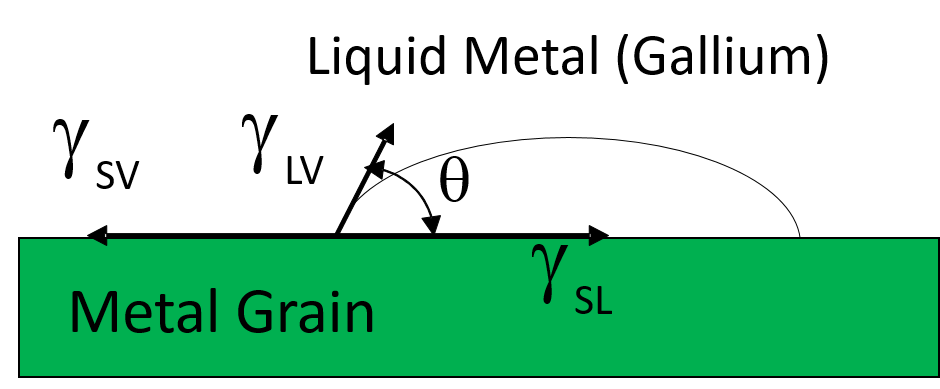
\includegraphics[width=\textwidth,trim={0 0 0 2cm}]{youngs-ga}
	%	\caption{Interfacial tensions on Ga drop on solid surface}
		\label{fig:youngs-ga}
	\end{subfigure}
	%add desired spacing between images, e. g. ~, \quad, \qquad, \hfill etc. 
	%(or a blank line to force the subfigure onto a new line)
	\begin{subfigure}[b]{0.5\textwidth}
		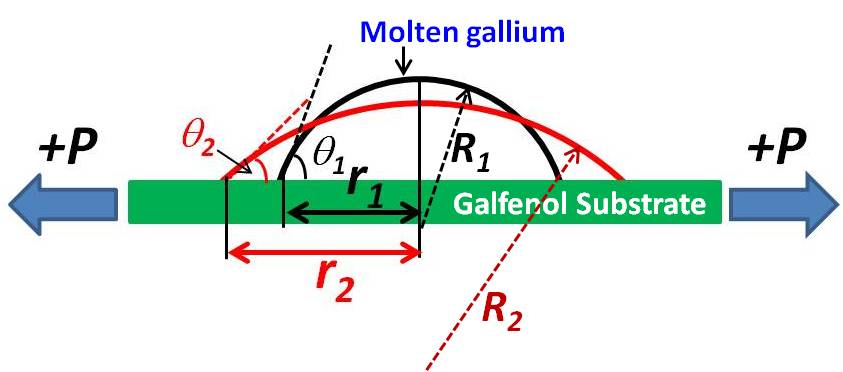
\includegraphics[width=\textwidth,trim={0 2cm 0 0}]{thermal-expand-drop}
	%	\caption{Thermal expansion of drop}
		\label{fig:thermal-expand-drop}
	\end{subfigure}
	\caption{Schematics indicating notation used and contact angles $\theta_{i}$, radii of drop-solid contact area $r_{i}$, and radii of curvature for a spherical drop $R_{i}$, for two temperatures as thermal expansion induced tension $P$ strains the substrate.}
	\label{fig:therm-exp-ga}
\end{wrapfigure}
The first technique that employs measurement of contact angles and drop size of a liquid metal, gallium, resting on a metal surface as the metal is heated. Changes in surface tension will be introduced by controlled thermal expansion of the substrate at temperatures ranging from $\sim$30-100\degree C to give mobility to the molten gallium drop.
% and ensure that surface heterogeneities do not obscure the drop-substrate contact angle. 
A video system to precisely quantify dimension changes in substrate and liquid metal drop during thermal expansion will be used. The surface energy of the free surface of the substrate as a function of temperature, \gamSV(T), can be related to thermal-expansion-induced changes in the liquid gallium drop contact angle $\theta$, the radius $r$ of the liquid gallium drop in contact with the metal surface, and the height $h$ of the hemisphere of liquid gallium. 

These can be modeled as a tensile load +$P(T)$ caused by substrate thermal expansion (Figure \ref{fig:therm-exp-ga}), which effectively appears as a uniform radial expansion of the planar solid surface as temperature increases. By letting the system equilibrate at different temperatures before measuring liquid drop geometry, terms due to variation in thermal energy and variation of the total Gibbs free energy vanish. Then, the interface energy between the substrate solid and the liquid gallium drop, \gamSL, is given as \gamSL$=P(T)/2\pi r$. The uniform tension introduced by thermal expansion of substrate can be expressed as:
\begin{equation}\label{uniform-tension}
	P(T) = E_{sub}\alpha_{sub}(T-T_{mp})
\end{equation}
where $T_{mp}$ is the melting temperature of gallium, $E$  is the substrate Young’s modulus, and $\alpha$ is the linear thermal expansion coefficient. A linear function can be used to write the gallium-air interfacial tension a function of temperature, \gamLV $= a-b(T-T_{mp})$, where \textit{a} and \textit{b} are positive constants found experimentally.\cite{Hardy1985,Alchagirov2005} Putting the terms for \gamSL and \gamSV into \hyperlink{youngeqn}{Young’s equation}\cite{Rudawska2009,Tadmor2004}:
\begin{equation*}%\label{youngs-eqn-ga1}
	\gamma_{SV} =  \frac{E_{sub}\alpha_{sub}(T-T_{mp})}{2\pi r} + \left[a-b(T-T_{mp})\right]\cos\theta
\end{equation*}

A relationship between the variable radius $r(T)$ associated with the area of the circular region of solid-liquid contact $A_{SL}(T)$, the contact angle $\theta(T)$ and the volume $V$ of the spherical cap formed by the drop is derived next. To determine the radius $r(T)$, the geometric relationships based on the radius of curvature $R(T)$ of a sphere is mapped onto the hemispherical liquid cap. The drop is modeled as being part of a sphere whose radius is $R(T)$. It is assumed that he volume $V$ of the drop is the volume of the spherical cap, and remains constant. The radius $R(T)$ can then be expressed in terms of the volume and the angle:
\begin{equation*}\label{drop-geom}
	R(T) = V^{1/3} \left[\frac{\pi}{3} \left(2-3\cos\theta(T)+\cos^{3}\theta(T)\right)\right]^{-1/3}
\end{equation*}
Using the relation $r(T)=R(T)\sin\theta(T)$ (i.e. $\theta=$0\degree corresponds to complete wetting of the surface and at $\theta=90$\degree,  $r=R$) the following formula for surface energy as a function of temperature $T$ and contact angle $\theta(T)$ (shown as $\theta_{T}$) is:
\begin{equation}\label{youngs-eqn-ga}
	\gamma_{SV} =  \underbracket{\frac{E_{sub}\alpha_{sub}(T-T_{mp})}{2\pi}\left[\frac{\pi\left(2-3\cos\theta_{T}+\cos^{3}\theta_{T}\right)}{3V\sin^{3}\theta_{T}} \right]^{1/3}}_{\text{\gamSL(T)}} + \underbracket{\left[a-b(T-T_{mp})\right]}_{\text{\gamLV(T)}} \cos\theta_{T}
\end{equation}
This gives the surface energy \gamSV of specific grains as a function of temperature by measuring $T$ and $\theta$ at thermal equilibrium.

One of the challenges in developing this new surface energy measurement capability is the need to expose the surface of the metal substrate shielded by surface oxides. The following strategies for removing of oxide layer and preventing of natural oxidation to increase the accuracy of measurement will be employed independently and in combination:
\begin{outline}
	\1 A flux used in high-temperature metal joining processes plays roles of dissolving of the oxides on the metal surface and preventing of re-oxidation as a chemical agent.
	\1 Colloidal silica polishing with nano-sized particles, such as is used for precise surface observations, like EBSD scans, which require clean surfaces to accurately detect patterns.
	\1 Electro-polishing is effective for passivation of clean surfaces after chemical and mechanical polishing for removal of surface oxides. 
\end{outline}
%Results using the proposed approach were to be validated through comparison of results for oriented single crystals with published theoretical values for pure metal elements of a specific crystallography (e.g. Ni, Cu, Fe)  and comparison with experimental data from amorphous metals (e.g. Vitreloy or liquid steel) with destructive high temperature methods for measuring surface energy. 
It should be noted that all of these techniques will not prevent oxides from forming for an extended period of time. Therefore, the cleaning would have to be followed by isolation in high vacuum, an inert environment, or another liquid environment that prevents oxidation.







%todo: Go through each version, and mark what was improved upon from experimental progression. 

\subsubsection{Thermal Grooving}

The thermal grooving technique was examined to provide a comparison point to our proposed gallium contact angle method.  These thermal grooves appear at grain boundaries, but the most information can be drawn from grain boundaries formed by two different crystal orientations. Using electron backscatter diffraction, EBSD, we identified grain orientations on samples of galfenol and alfenol to identify the grain boundaries where \hkl(100), \hkl(110), and \hkl(111) orientations met.  By measuring the dihedral angle formed at these grain boundaries after polishing and annealing, we calculated the ratio of grain boundary energy and surface energy according to the following equation: 

\begin{figure}[h]
	\centering
	\begin{subfigure}[c]{0.45\textwidth}
		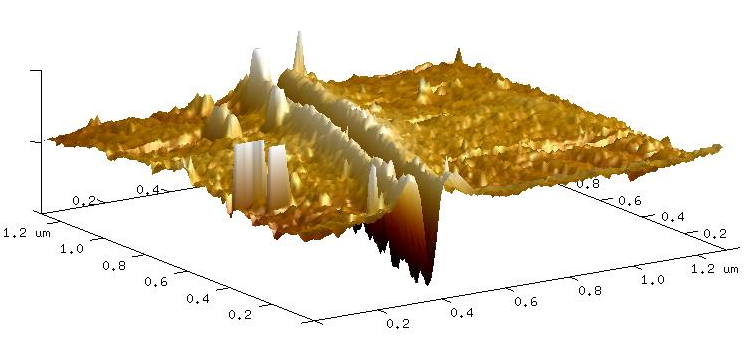
\includegraphics[width=\linewidth]{afm-groove-fega}
		\subcaption{~}
		\label{fig:afm-groove-fega}		
	\end{subfigure}
	\begin{subfigure}[c]{0.45\textwidth} 
		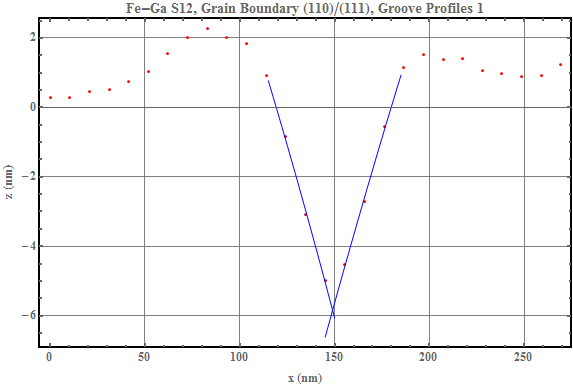
\includegraphics[width=\linewidth]{fega-groove-profile}
		\subcaption{~}
		\label{fig:fega-groove-profile}		
	\end{subfigure}
	\caption{(a) 3D rendering of (110)/(111) grain boundary on surface of  for (Fe-19\%Ga)+1.0\%NbC sample where the depth of groove is ~8 nm. (b) A quadratic fit of a (110)/(111) grain boundary profile for a (Fe-19\%Ga)+1.0\%NbC sample.}
	\label{fig:thermal-groove}
\end{figure}
\begin{equation}
	\frac{\gamma_{GB}}{\gamma_{S}} = 2\cos\left(\frac{\Psi_{S}}{2}\right) 
\end{equation}
where $\gamma_{GB}$ is the grain boundary energy, $\gamma_{S}  $ is the surface energy, and $\Psi_{S} $ is the dihedral angle, as described in Rohrer et al.\cite{Rohrer2010a} The most symmetric thermal groove came from a \hkl(110)/\hkl(111) grain boundary on a rolled and annealed (Fe-19\%Ga)+1.0\%NbC sample made by Suok-Min Na, as seen in the Figure \ref{fig:thermal-groove}.  The grain boundary profiles were measured using atomic force microscopy (AFM), and the dihedral angles were extrapolated from the profiles using both AFM software by Bruker and, the more accurate, quadratic fit.  The results are shown in Table \ref{groove-analysis}.  This groove in particular had a depth of $\sim$8 nm which is significantly smaller in depth compared to grooves of other metal alloys in literature.  Also, many of the grain boundary grooves were not suitable for measuring based on their lack of symmetry at the grain boundary interface. It is worthy to note that this technique is very time consuming and slightly destructive to the surface. To properly analyze the thermal grooving technique, an extensive grain boundary study of annealing temperatures and times on Alfenol and Galfenol would have to be carried out. While this may be an interesting avenue of research in the future, the resultant calculations of relative grain energies does not benefit our ultimate goal of achieving a comprehensive AGG model for Galfenol and Alfenol. Realization of our goal lies in the measurement of orientation-dependent surface energy using contact angle measurements. 


\begin{table}[h!]
	\centering
	\caption{Calculated dihedral angles and relative energies from our most symmetric grain boundary groove.}
	\begin{tabular} { |p{1cm}||c|c|c|c|  } 
		\hline
		\multicolumn{5}{|c|}{fe-ga-s12-006 profile analysis - GB (110)/(111)}\\
		\hline
		~	&\multicolumn{2}{|c|}{Bruker Software}		&\multicolumn{2}{|c|}{Quadratic Fit}	\\
		\hline
		Profile	&Dihedral Angle (\degree)	&Relative Energy	&Dihedral Angle (\degree)	&Relative Energy \\ 
		\hline
		1		&156.957	&0.399471	&151.253	&0.496475	\\
		\hline
		2		&156.244	&0.411657	&157.093	&0.397144	\\
		\hline
		3		&154.402	&0.443063	&155.554	&0.423432	\\
		\hline
		4		&157.221	&0.394955	&152.785	&0.470541	\\
		\hline
		5		&154.732	&0.437445	&154.966	&0.433458	\\
		\hline
		6		&158.386	&0.375003	&154.482	&0.441706	\\
		\hline
		\textbf{Avg}	&156.324~$\pm$1.529	&0.410266 $\pm$0.0261178	&154.356 $\pm$2.069	&0.443793 $\pm$0.0351932\\
		\hline
	\end{tabular}
	\label{groove-analysis}
\end{table}

	


\subsubsection{Contact Angle Goniometer (Verison 1)}
Preliminary designs of our contact angle goniometer implement a radiative temperature control box which encloses an argon gas filled container where the sample resides, as seen in Figure \ref{fig:rad-temp-box}.  The presence of argon is meant to prevent any further oxidation of the Galfenol sample as well as the gallium droplet. The argon filled container was initially made of a clear acrylic plastic, but prolonged exposure to temperatures above 80\degree C caused thermal deformation of the plastic making longer experiments impossible to perform without environment contamination.  A clear pyrex container replaced the acrylic box to fix this issue.  Application of the liquid gallium drop to our surfaces was done via a mounted plastic syringe with commercially available disposable stainless steel hypodermic needles.  Observations of this application show that the hypodermic needles present multiple problems to the sessile drop method.  Liquid gallium tends to adhere strongly to the stainless steel needle tips which makes wetting to the sample very difficult.  Tapping the syringe will remove the drop needle and allow gallium to wet the surface, but this is not ideal because the additional dropping force from gravity will cause further spreading not associated with the intrinsic surface energy of the substrate.  Also, the angled hypodermic tip tends to deform the highly viscous gallium drop resulting in non-uniform hemispheric drop shapes, as shown in Figure \ref{fig:deformed-ga}.
\begin{figure}
	\centering
	\begin{subfigure}[c]{0.45\textwidth}
		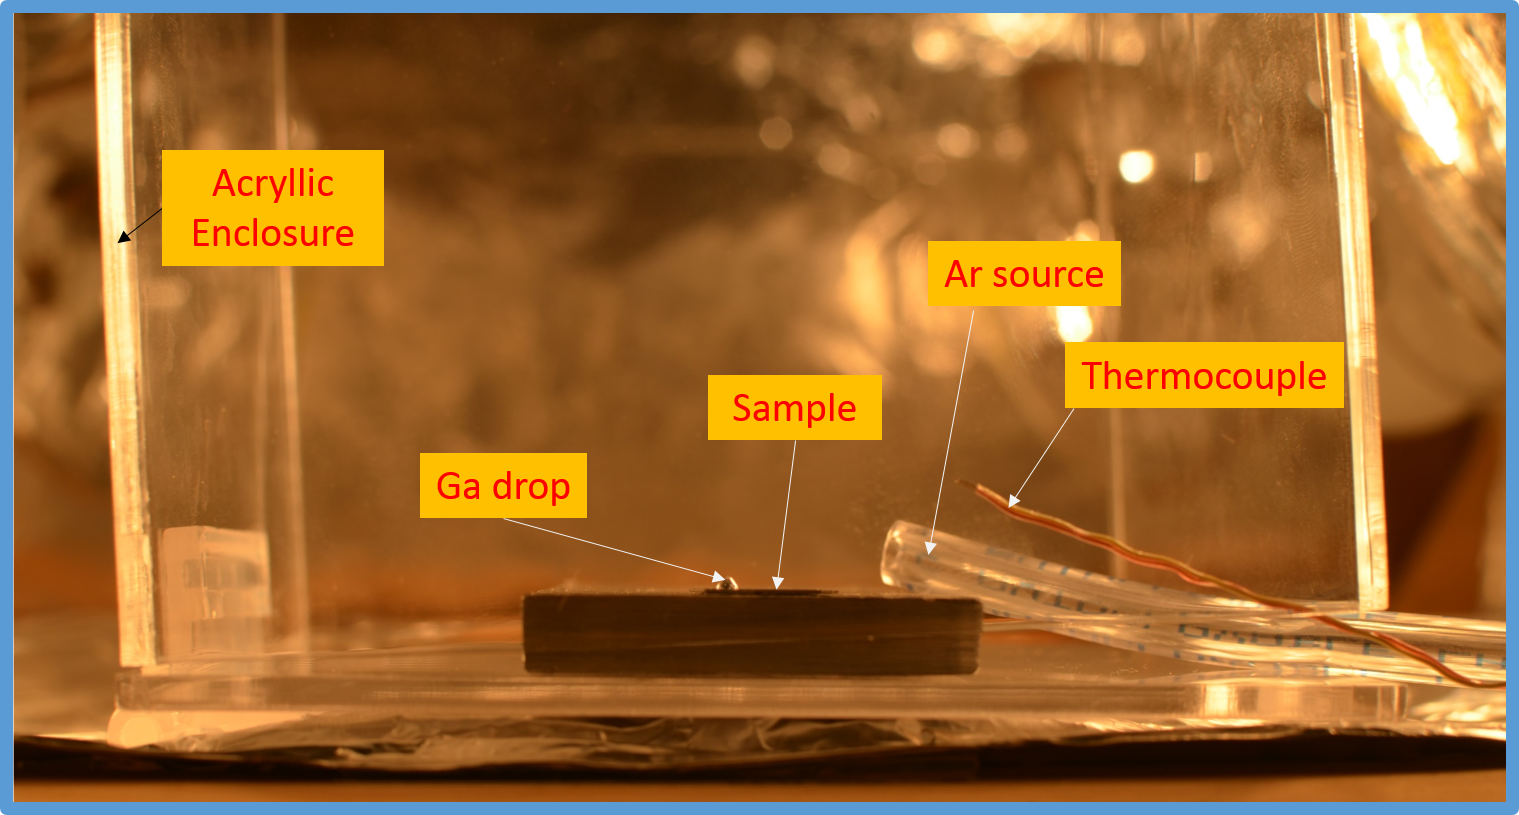
\includegraphics[width=\linewidth]{rad-temp-box}
		\subcaption{~}
		\label{fig:rad-temp-box}		
	\end{subfigure}
	\begin{subfigure}[c]{0.45\textwidth} 
		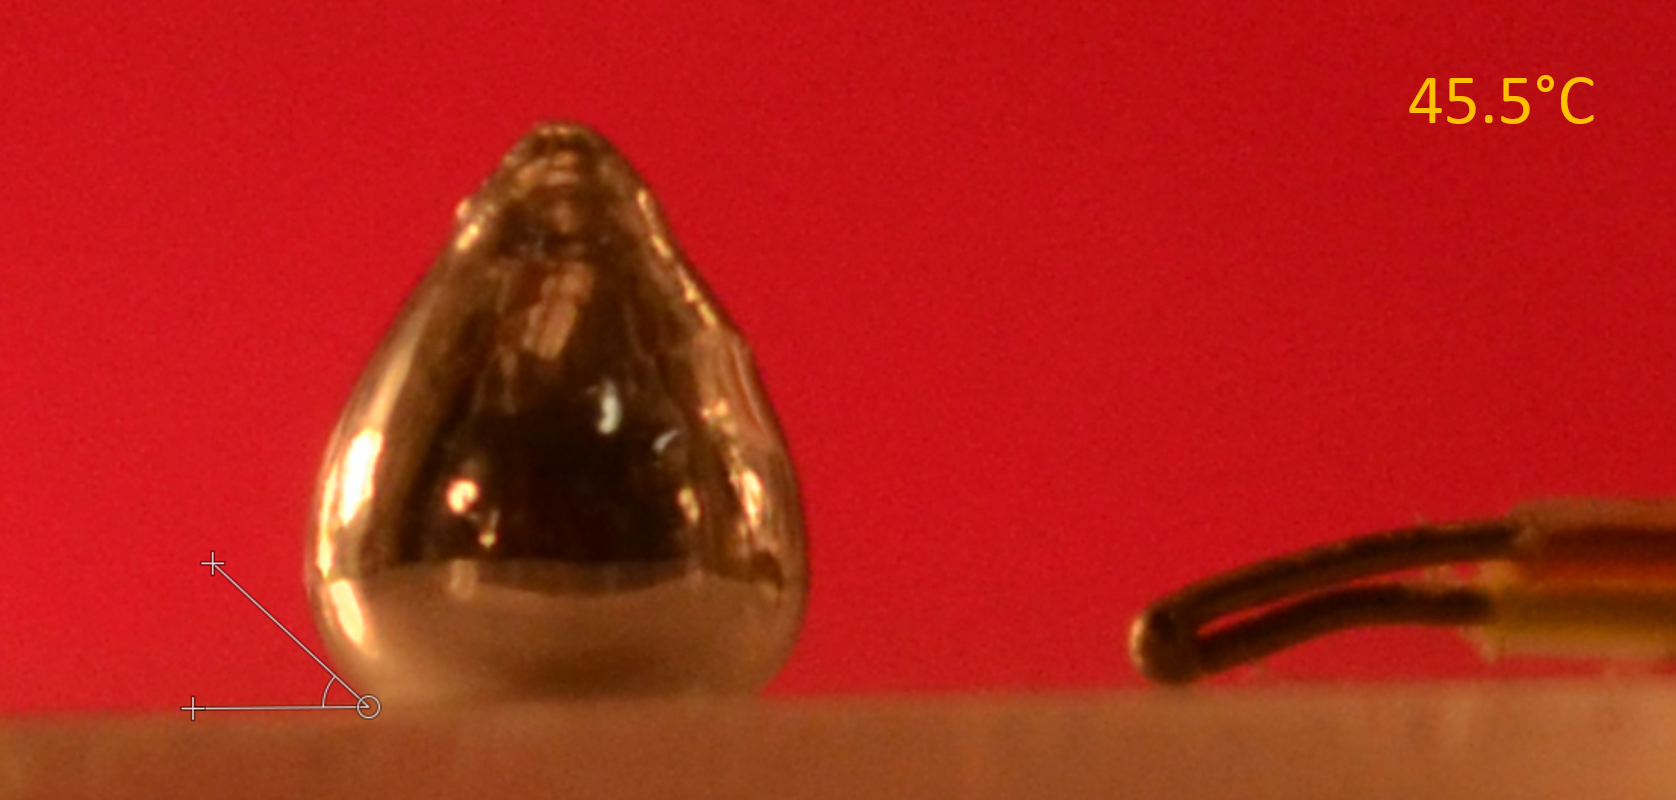
\includegraphics[width=\linewidth]{deformed-ga}
		\subcaption{~}
		\label{fig:deformed-ga}		
	\end{subfigure}
	\caption{(a) The first design of our contact angle goniometer.  The acrylic container houses the argon environment and sample.  This design was modified with a more stable glass enclosure. (b) A highly deformed gallium drop next to the thermocouple on a ceramic YAG test sample at 45.5\degree C.}
	\label{fig:prelim-design}
\end{figure}

For this experiment to succeed, a number of challenges were overcome. The simplest task involved polishing Galfenol samples using incrementally higher grit SiC paper and subsequent 0.1 $\mu$m colloidal silica particles to decrease the roughness to below 40 nm, as proven using AFM measurements. %TODO: Find AFM roughness picture?
% AFM roughness pic
%\begin{figure}
%	\centering
%		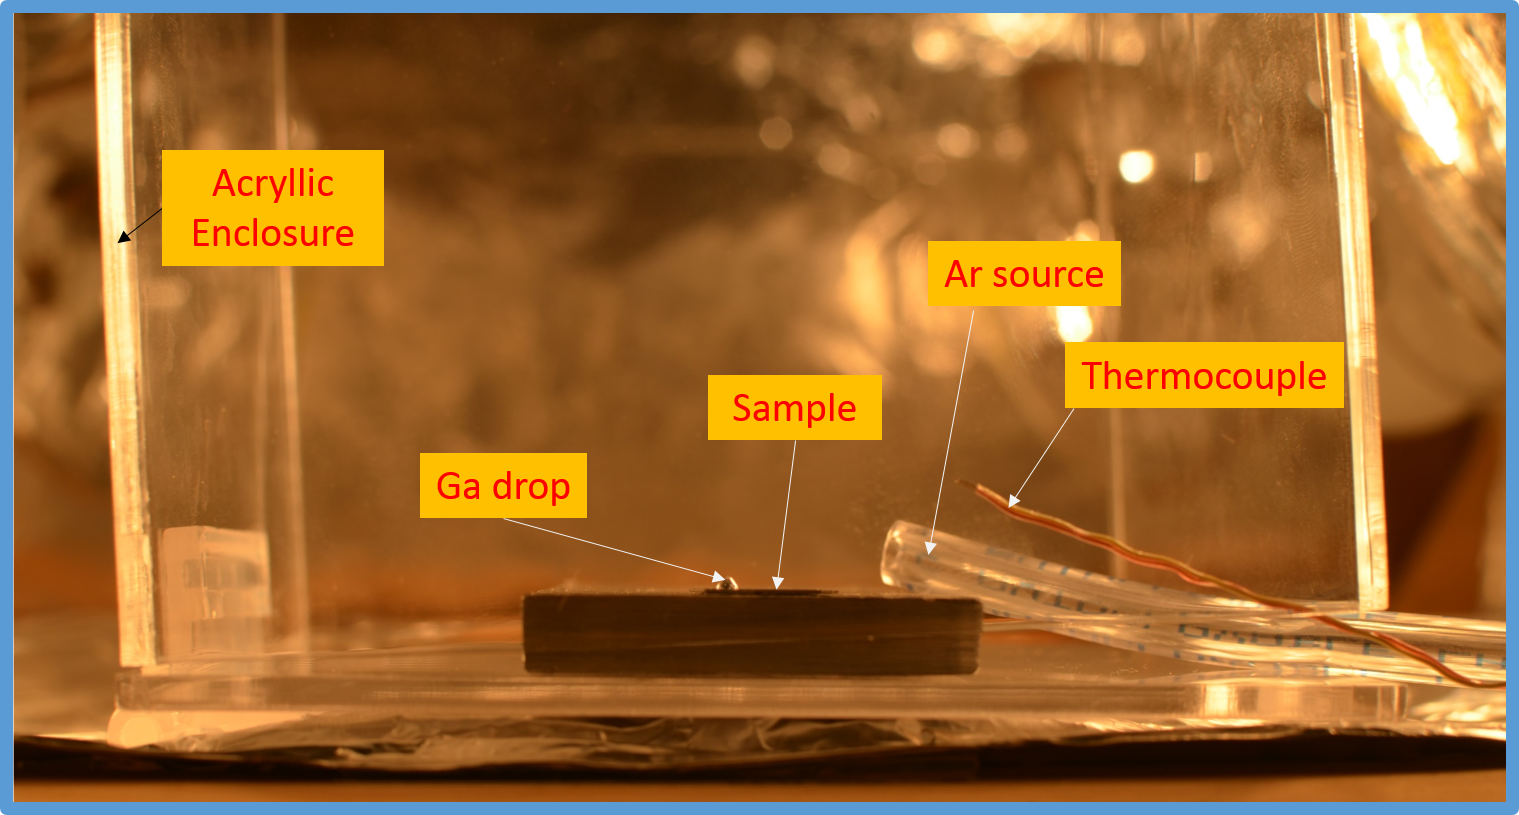
\includegraphics[width=\linewidth]{rad-temp-box}
%	\caption{(a) The first design of our contact angle goniometer.  The acrylic container houses the argon environment and sample.  This design was modified with a more stable glass enclosure. (b) A highly deformed gallium drop next to the thermocouple on a ceramic YAG test sample at 45.5\degree C.}
%	\label{fig:prelim-design}
%\end{figure}

The radiative box that housed this experiment had a high variability in temperature caused by opening and closing the box when interaction with the gallium dispensing syringe was needed. A smaller apparatus with a top-side syringe opening is needed to properly perform gallium drop tests at specific temperatures and prevent interaction with the experiment environment. There must also be bright white backlighting to obtain a high contrast drop profile. In this radiative box configuration, the high-reflecting liquid metal surface prevents a high contrast drop profile image, as seen in Figure \ref{fig:deformed-ga}. Proper contact angle measurements also require the gallium droplets to carefully wet the surface while forming an axisymmetric and spherical-like shape on the solid surface. A height adjustment system must be used to move the gallium pendant drop close enough to the sample surface for solid adhesive forces to overcome the adhesion to the needle. Lastly, the argon gas environment could be more well contained, instead of just filling up the glass sample enclosure from the bottom and spilling out the top. This occurs because argon has a higher density than the surrounding air environment. 

\subsubsection{Version 2}


Most of the issues associated with Version 1 of are addressed in Version 2 of the gallium drop experiment. The new experimental apparatus can be seen in Figure \ref{fig:enviro_chamber}. The main structure is made of aluminum with two round glass windows on the front and back. The aluminum
\begin{wrapfigure}[11]{r}{0.5\linewidth}
	\centering
	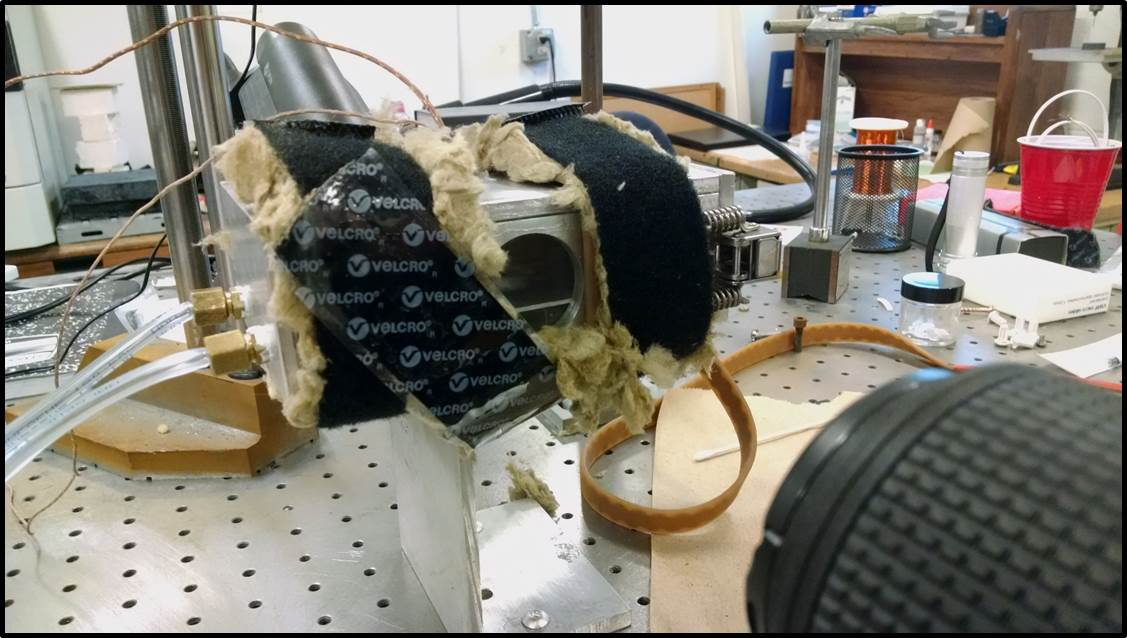
\includegraphics[width=\linewidth,trim={0 0 0 0}]{enviro_chamber}
	\caption{The second version of our gallium contact angle goniometer. The aluminum enclosure conductively transfers heat, the gas lines flow Ar gas into the chamber, top-mounted thermocouples monitor the gas and sample temperature, and the glass windows allow for backlighting of the drop profile along with high resolution image capture using a DSLR camera.}
	\label{fig:enviro_chamber}
\end{wrapfigure}
 is meant to conductively transfer heat to the substrate by means of a heating cable wrapped around the outside of the structure. The high thermal conductivity of aluminum allows for a quick transfer of heat, thus an increased control of sample temperature using the heating tape. The time percentage dial controller attached to the heating tape is calibrated with the sample temperature using a thermocouple placed on the sample surface. Sample temperature can be consistently controlled with $\pm$0.5\degree C accuracy. Backlighting greatly improved the drop profile contrast by having only one white light source coming from one side of the droplet, as seen in Figure \ref{fig:deformed_ga}. The Ar environment is also far more contained and controlled. The silicone sealant creates a nearly air-tight system where the argon will displace all gas contaminants that could oxidize the sample or gallium droplet. These precautions are suitable for any metals samples we test because each sample is polished according to the procedure described above and then cleaned with acetone to remove any oxides. Once the sample is inserted and sealed in the environmental chamber, the Ar prevents oxidation throughout the experiment. A positive partial pressure is achieved in the chamber with an in- and out-valve. %TODO find more sufficient answer to how this removes oxides. 

\begin{wrapfigure}[8]{R}{0.5\linewidth}
	\centering
	\begin{subfigure}[c]{0.22\textwidth}
		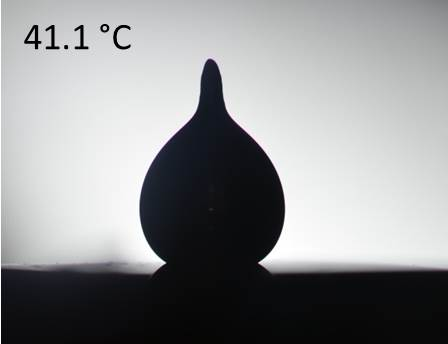
\includegraphics[width=\linewidth,trim={0 0 0 0}]{ga_41c}
		\subcaption{~}
		\label{fig:ga_41c}		
	\end{subfigure}
	\begin{subfigure}[c]{0.23\textwidth} 
		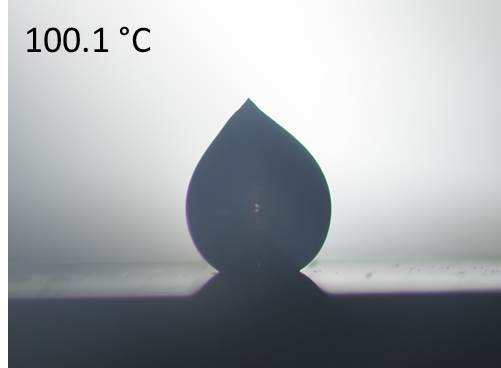
\includegraphics[width=\linewidth,trim={0 0 0 0}]{ga_100c}
		\subcaption{~}
		\label{fig:ga_100c}		
	\end{subfigure}
	\caption{Pure liquid gallium obtains viscoelastic properties when trace amounts of oxygen are present via formation of oxide shell. Non-axisymmetric Ga drops form on this iron substrate}
	\label{fig:deformed_ga}
\end{wrapfigure}

While extensive steps have been taken to inhibit oxidation of our metal samples, preventing oxidation on the surface of liquid gallium was a greater challenge. Pure gallium and Gallium-based alloy surfaces instantly oxidize in ambient environments, turning into a thin layer of gallium oxide (Ga$_{2}$O$_{3}$ and Ga$_{2}$O).\cite{Regan1995,Regan1997,Scharmann2004} This oxide layer is solid and remains elastic until it experiences a yield stress. Therefore, that an oxidized gallium droplet does not behave as a simple liquid, but as a viscoelastic material. In addition, the oxide layer of gallium is known to adhere to almost any solid surface, causing a severe stiction problem that interferes with interfacial energy measurements.\cite{Scharmann2004}. This shows how dramatically the gallium surface tension decreases when the oxide forms. Khan et al. showed that gallium oxide forms hydroxyl groups on their exterior surface, making the drops lyophilic as opposed to the expected lyophobic behavior of pure gallium, a high surface tension liquid.\cite{Hardy1985,Alchagirov2005} 


Figure \ref{fig:deformed_ga} shows our direct observation of this phenomenon with teardrop shaped droplets formed by adhering to the iron surface while still being pulled upwards by the deposition needles. The general shape of these drops were unchanged for many hours even at temperatures approaching $\sim$100\degree C, thus exhibiting the stability of viscoelastic properties caused by the solid oxide layer. Removing the oxide layer from liquid gallium will return normal liquid properties to gallium and allow the use of axisymmetric drop analysis calculations: Young-Laplace equation, 
%todo: [NEED MORE TECHNIQUES FROM KRUSS GONIOMETER]



Oxide removal permits liquid gallium to directly interact with metal surfaces instead of gallium oxide; the derived terms for \gamSL and \gamLV in Equation \ref{youngs-eqn-ga} become more robust. A number of techniques have been developed to remove and recover gallium oxide on liquid gallium: ultra-high vacuum (UHV) techniques,\cite{Regan1995,Regan1997} chemical vapor etching,\cite{Kim2013,Doudrick2014} and electrohydrodynamic phenomena.\cite{Khan2014} A chemical vapor etch is the best option for our purposes because it has a minimal effect on the surface of metals and the experimental apparatus does not need to be changed. To execute the vapor etch, a pendant drop of gallium was formed and a pipette of 37wt\% HCl was brought in close proximity to etch away the oxide layer. The same procedure was performed on the sessile drop of gallium on the desired surface to etch away any oxide left on top of the droplet, as seen in Figure \ref{fig:hcl_vapor_treat}. The contact angles of gallium on bare glass before and after HCl vapor treatment are similar to respective contact angle values in Kim et al.\cite{Kim2013}

\begin{wrapfigure}[8]{L}{0.6\linewidth}
	\centering
	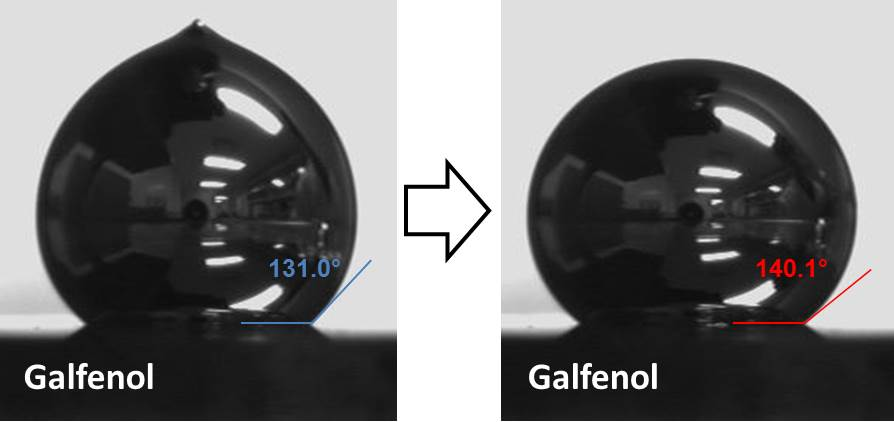
\includegraphics[width=\linewidth,trim={0 0 0 1cm}]{hcl_vapor_treat}
	\caption{This image shows the contact angle of gallium on a bare glass slide in an argon environment before and after HCl vapor treatment.}
	\label{fig:hcl_vapor_treat}
\end{wrapfigure}

With the HCl vapor treatment added to the procedure, temperature-varying gallium contact angle measurements in an argon environment were executed in the aluminum chamber on multiple metal substrates. Polycrystalline samples of high quality ($>$99.99\%) tin, copper, and iron were polished and had liquid gallium deposited on their surfaces. The temperature in the chamber was slowly ($<$10\degree C/min) increased from ~30\degree C to just below 100\degree C. Beyond 100\degree C, the heating tape becomes inconsistent with the intervals of heat applied to the chamber. Photographs of the gallium drops profiles are taken at ~10\degree C intervals to observe progression of the drop shape as temperature increases. The same procedure is done as the temperature is decreased to 30\degree C to observe reversibility of this process, since we assume that the thermal expansion of the substrate drives the change in \gamSL from Equation \ref{youngs-eqn-ga}. 

It is known that liquid gallium tends to corrode most metal surfaces.\cite{Lewandowski2015,Narh1998,Fitzgerald1999} Since experiments lasted for less than one hour, corrosion between the two metals would not be significant enough to effect the measurement. For the tin and copper samples, gallium began to visibly corrode through the surface between 60\degree C and 70\degree C, as evident by a rapid contact angle decrease on only side of the drop profile. The iron sample did not have any corrosion problems throughout the experiments. It is expected that as the temperature increases, the thermal expansion of the solid will isotropically expand the drop thus decreasing the contact angle. Some gallium contact angles decrease on iron, but it is often that the decrease occurs on one side of the drop profile as the temperature increases. We believe that this is due to the polycrystalline grains having different thermal expansions, hence the drop spreading is anisotropic. This proves that a single crystal grain or abnormally grown surface grain is needed to properly observe an isotropic drop expansion. 

\begin{wrapfigure}[8]{R}{0.5\linewidth}
	\centering
	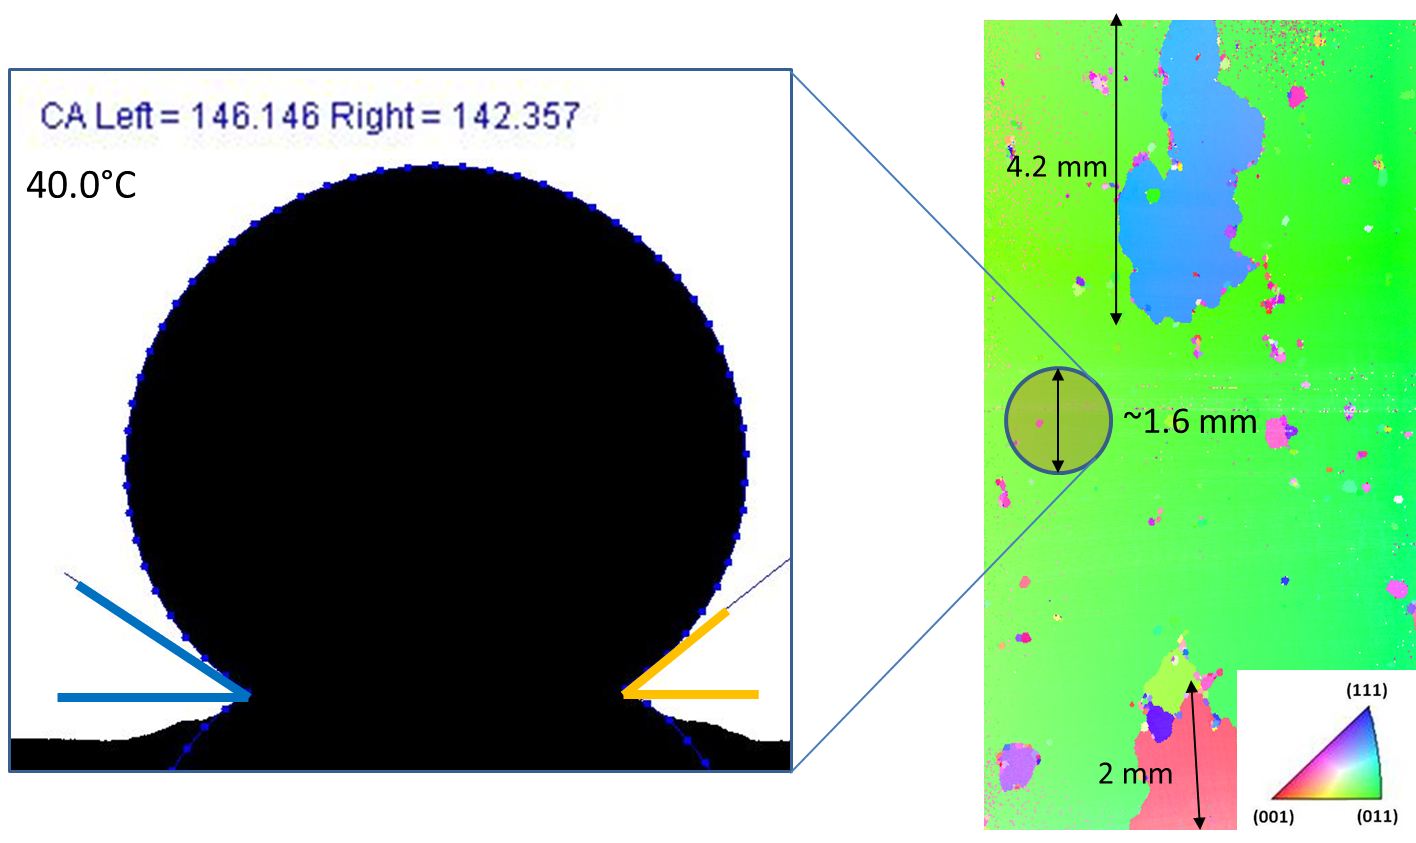
\includegraphics[width=\linewidth,trim={0 0 0 1.5cm}]{ca_ebsd}
	\caption{The location of a gallium drop on highly Goss-textured surface.}
	\label{fig:ca_ebsd}
\end{wrapfigure}

Since the iron sample did not corrode in the presence of gallium, we proceeded to a Galfenol sample with an abnormally grown \hkl(110) grain. Figure \ref{fig:ca_ebsd} shows the location of a gallium droplet in contact with the highly Goss-textured surface. Using the same temperature intervals, the right and left contact angles were measured and the surface energy was calculated using Equation \ref{youngs-eqn-ga}. The contact angle measurements and surface energy calculations are shown in Figure \ref{fig:goss_se_msrmnt}. The contact angle measurements clearly show anisotropic spreading behavior since the left contact angle recedes as temperature increases while the right contact angle advances. At 60.7\degree C, the contact angles reached close to the same value which may indicate an equilibrium point of combating thermal expansions caused by nearby island grains. 

We did not expect to see an increasing surface energy trend as the temperature increased. As the temperature of a metal surface increases, the cohesive force binding atoms will decrease because the atoms will vibrate more rapidly. Since surface energy depends on the net inward cohesive force, we should see a decrease in surface energy with increasing temperature. Moreover, we did not expect such a high difference in surface energy as the temperature increased. The values of surface energy for the \hkl(110) Galfenol grain are two orders of magnitude greater than predicted values of $\alpha$-iron, \gamSV = 2.0535 J/m$^2$.\cite{Wang2000} After presenting our findings at the XXIV International Materials Research Congress and 2015 MRS Fall Meeting,\cite{VanOrder2015a,VanOrder2015} we discussed possible avenues of improvement for the gallium contact angle experiment with colleagues and potential collaborators. A more concrete measurement of \gamSL between liquid gallium and solid would need to be examined, a very non-trivial task. Ultimately, we decided to suspend the gallium drop experiment and re-evaluate our strategy for obtaining orientation-dependent surface energies of magnetostrictive materials. 

\begin{figure}[h]
	\centering
	\begin{subfigure}[c]{0.47\textwidth}
		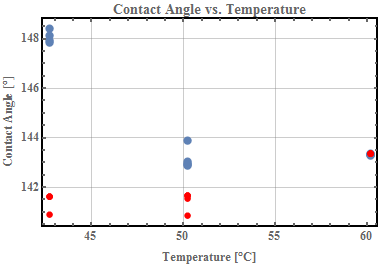
\includegraphics[width=\linewidth]{goss_ga_ca}
		\subcaption{~}
		\label{fig:goss_ga_ca}		
	\end{subfigure}
	\begin{subfigure}[c]{0.47\textwidth} 
		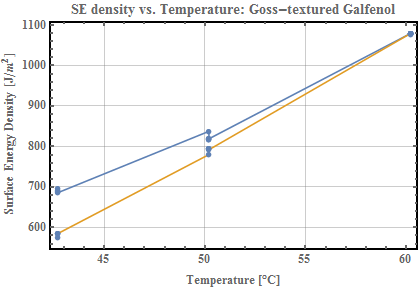
\includegraphics[width=\linewidth]{goss_ga_se}
		\subcaption{~}
		\label{fig:goss_ga_se}		
	\end{subfigure}
	\caption{(a) Blue and red dots show left and right contact angle, respectively, of liquid gallium on \hkl(110) Fe-Ga. (b) Calculated surface energy values of \hkl(110) Fe-Ga grains using Equation \ref{youngs-eqn-ga}.}
	\label{fig:goss_se_msrmnt}
\end{figure}

Overall, this was an exploration of well-proposed and innovative research. We made assumptions about how the system would interact and tried to yield good results in the lab. We found that these assumptions were too great and the experiment failed to meet expectations. Much was learned about the complexity of surface energy research from both a theoretical and experimental perspective. This failure persuaded us to find a more robust and promising method for accomplishing our goal within our constraints of non-destructive orientation-dependent surface energy characterization. 


%\begin{outline}[enumerate]
%	\1 Radiative box [X]
%		\2 Plexiglass chamber [X]
%		\2 Glass chamber [X]
%		\2 Low control of temperature and image clarity [X]
%			\3 Need temperature control and backlighting, while improving gas environment. [X]
%	\1 Aluminum conductive environmental chamber [X]
%		\2 Deformed droplets persist and contact angle cannot be properly measured [X]
%		\2 HCl etching to achieve axisymmetric gallium drops [X]
%		\2 Surface energy is be measured [X]
%		
%	\1 MRS Fall Meeting [~]
%		\2 Learning from wetting dynamics community [X]
%			\3 Static contact angles are not well accepted due to inconsistency  [X]
%			\3 make connections to wetting dynamics research group in UMD Mechanical Engineering [X] 
%			\3 Learn that gallium drop model is incorrect on a thermodynamic equilibrium level [X]
%				\4 Using one thermodynamic equilibrium equation and then plugging values into another thermodynamic equilibrium equation [X]
%		
%\end{outline}


%\subsection{Results and Presentations}

%TODO: Explain why this method is not possible from a fundamental thermodynamic position (ie using one thermodynamic equilibirum and plugging it in to another equation at thermodynamic equilibrium). Should be able to go from one thermodynamic equilibrium equation to another, but that is not the case here. The method could still be feasible if more terms (\gamSL between liquid-Ga and solid) were known
